\documentclass{article}
% packages used

\usepackage{amsmath}
\usepackage{amssymb}
\usepackage{amsfonts}
\usepackage{amsthm}
\usepackage{bm}
\usepackage{graphicx}
\usepackage{cite}

% fonts used
%\usepackage{fourier}
\usepackage{nimbusmononarrow}
\usepackage{microtype}
%\usepackage{fontspec}
%\setsansfont{Linux Biolinum}
%\setmonofont{Linux Mono}
% theorems, remarks, etc
  %% types italiques
\theoremstyle{plain}
\newtheorem{lemma}{Lemma}[section]
\newtheorem{proposition}{Proposition}[section]
\newtheorem{theo}{Theorem}[section]
\newtheorem{algo}{Algorithm}[section]
\newtheorem{assump}{\bf{Assumption}}[section]
\newtheorem{conj}{Conjecture}[section]
  %% types roman
\theoremstyle{remark}
\newtheorem{remark}{\bf{Remark}}[section]
\theoremstyle{remark}
\newtheorem{example}{\bf{Example}}[section]
\theoremstyle{remark}
\newtheorem{definition}{\bf{Definition}}[section]
  %\newtheorem{appendix}{\bm Definition}[section]


%------------------------------------------------------------------------
%--------------------------- personal macros ---------------------------
%------------------------------------------------------------------------

%\renewcommand{\theequation}{\arabic{section}.\arabic{equation}}
\numberwithin{equation}{section}

\newcommand*\diff{\mathop{}\!\mathrm{d}}
\newcommand*\Diff[1]{\mathop{}\!\mathrm{d^#1}}

%----- typos
\newcommand{\ie}{{\it i.e. \/}}

%----- fractions
\newcommand{\half}{\frac{1}{2}}

%---- bold characters
\newcommand{\bx}{{\bf{x}}}
\newcommand{\by}{{\bf{y}}}
\newcommand{\bk}{{\bf{k}}}
\newcommand{\bz}{{\bf{0}}}

%----- set
\newcommand{\R}{{\mathbb{R}}}
\newcommand{\Z}{{\mathbb{Z}}}
\newcommand{\N}{{\mathbb{N}}}
\newcommand{\Nm}{{\mathcal{N}}}
\newcommand{\RN}{\R^{\N}}
\newcommand{\p}{\mathcal{P}}

%----- derivatives
\newcommand{\dt}{\partial_t}
\newcommand{\dx}{\partial_x}
\newcommand{\dxx}{\partial_{xx}}
\newcommand{\dyy}{\partial_{yy}}
\newcommand{\dtt}{\partial_{tt}}
\newcommand{\dtx}{\partial_{tx}}
\newcommand{\dxtt}{\partial_{xtt}}
\newcommand{\dtxx}{\partial_{txx}}
\newcommand{\grdx}{\nabla_x}

\newcommand{\dz}{\partial_z}
\newcommand{\dnz}[1]{\partial^{#1}_z}

%----- greek letters
\newcommand{\eps}{\varepsilon}


%------------------------------------------------------------------------
%----------------------- end of personal macros ------------------------
%------------------------------------------------------------------------


\begin{document}

% \begin{flushright}
%   {\it draft, \today}
% \end{flushright}
%\begin{center}
\title{Notes}

\author{}
%\end{center}

\maketitle

\section{Formulation and Algorithm}

We are interested in the steady state, namely, the minimizer of the following energy functional:
\begin{equation}\label{origin_energy}
  E(m) = \frac{1}{2}\int_\Omega \left(D^2|\nabla m|^2 + \frac{\alpha}{\gamma}|m|^{2\gamma} + c^2|m\cdot\nabla p|^2 + c^2r(x) |\nabla p|^2\right) \diff x,
\end{equation}
with the following constrain:
\begin{equation}\label{origin_constrain}
  -\nabla\cdot\left((r^2 I + m\otimes m)\nabla p\right) = S.
\end{equation}

First by introducing a new variable $q$ satisfying
\begin{equation}
  q = (m\otimes m) s,
\end{equation}
the the functional~\eqref{origin_energy} can be written as
\begin{equation}\label{origin_energy}
  E(m) = \frac{1}{2}\int_\Omega \left(D^2|\nabla m|^2 + \frac{\alpha}{\gamma}|m|^{2\gamma} + q\cdot s + c^2r(x) |\nabla p|^2\right) \diff x,
\end{equation}
also for the constrain~\eqref{origin_constrain},
\begin{equation}
  -r^2\nabla \cdot s - \nabla\cdot q = S.
\end{equation}.

So now we want to solve the following constrained optimization problem:
\begin{align}
  &\min_{m,\nabla p,q}
  \frac{1}{2}\int_\Omega\left(D^2|\nabla m|^2 + \frac{\alpha}{\gamma}|m|^{2\gamma} + q\cdot s + c^2r(x) |\nabla p|^2\right) \diff x \\
  \text{such that: } &-r^2\nabla\cdot s - \nabla\cdot q = S, \\
  &q = (m\otimes m)s
\end{align}
Algorithm: denote $E(m, s, q)$ as energy:
\begin{multline}
  \frac{1}{2}\int_\Omega D^2|\nabla m|^2 + \frac{\alpha}{\gamma}|m|^{2\gamma} + q\cdot s + c^2r(x) |\nabla p|^2 \\
  + \lambda |r^2\nabla\cdot s + \nabla\cdot q + S|^2 + \lambda|q - (m\otimes m) s|^2 \diff x.
\end{multline}

\begin{align}
  &(m^{k+1}, s^{k+1}, q^{k+1}) = \arg\min_{m,s,q} E(m, s, q) - \langle p^k_m, m - m^k \rangle - \langle p^k_s, s - s^k \rangle - \langle p^k_q, q - q^k \rangle \\
  &p^{k+1}_q = p^k_q - \lambda \nabla (r^2\nabla\cdot s^{k+1} + \nabla\cdot q^{k+1} + S) - \lambda (q^{k+1} - (m^{k+1}\otimes m^{k+1})s^{k+1}) \\
  &p^{k+1}_s = p^k_s - \lambda \nabla (r^4\nabla\cdot s^{k+1} + r^2\nabla\cdot q^{k+1} + r^2S) \\
  & - \lambda (m^{k+1}\otimes m^{k+1})((m^{k+1}\otimes m^{k+1})s^{k+1} - q^{k+1}) \\
  &p^{k+1}_m = p^k_m - \lambda (s^{k+1}\otimes m^{k+1} + s^{k+1}\cdot m^{k+1} I)((m^{k+1}\otimes m^{k+1})s^{k+1} - q^{k+1})
\end{align}
Define
\begin{equation}
  F(m) = \frac{1}{2}(\frac{\alpha}{\gamma}|m|^{2\gamma} +  \lambda|q - (m\otimes m) s|^2),
\end{equation}
\begin{equation}
  E_1 = \int_\Omega F(m)\diff x, \quad v(t) = \sqrt{E_1}.
\end{equation}
The dynamics of this system is
\begin{align}
  \frac{\partial m}{\partial t} = -D^2\Delta m + \frac{v(t)}{\sqrt{E_1(m)}}F'(m)\\
  v_t(t) = \frac{1}{2\sqrt{E_1(m)}}\int_\Omega F'(m)m_t\diff x.
\end{align}

\section{Introduction}
$dx = dy = 0.01$, $dt = 0.005$, $T = 1$. $r = 0.1$, $c = 50$, $D = 0.001$, $\rho = 10^{-12}$ and $\gamma = 0.75$.
\begin{figure}
  \includegraphics[width=0.5\textwidth]{1/m1}
  \includegraphics[width=0.5\textwidth]{1/s}
\end{figure}
\begin{figure}
  \includegraphics[width=0.5\textwidth]{1/PCG}
  \includegraphics[width=0.5\textwidth]{1/vector}
\end{figure}

\begin{figure}
  \includegraphics[width=0.5\textwidth]{2/m1}
  \includegraphics[width=0.5\textwidth]{2/s}
\end{figure}
\begin{figure}
  \includegraphics[width=0.5\textwidth]{2/PCG}
  \includegraphics[width=0.5\textwidth]{2/vector}
\end{figure}
\begin{figure}
  \includegraphics[width=0.5\textwidth]{3/m1}
  \includegraphics[width=0.5\textwidth]{3/s}
\end{figure}
\begin{figure}
  \includegraphics[width=0.5\textwidth]{3/PCG}
  \includegraphics[width=0.5\textwidth]{3/vector}
\end{figure}
\begin{figure}
  \includegraphics[width=0.5\textwidth]{4/m1}
  \includegraphics[width=0.5\textwidth]{4/s}
\end{figure}
\begin{figure}
  \includegraphics[width=0.5\textwidth]{4/PCG}
  \includegraphics[width=0.5\textwidth]{4/vector}
\end{figure}
\begin{figure}
  \includegraphics[width=0.5\textwidth]{5/m1}
  \includegraphics[width=0.5\textwidth]{5/s}
\end{figure}
\begin{figure}
  \includegraphics[width=0.5\textwidth]{5/PCG}
  \includegraphics[width=0.5\textwidth]{5/vector}
\end{figure}
\begin{figure}
  \includegraphics[width=0.5\textwidth]{6/m1}
  \includegraphics[width=0.5\textwidth]{6/s}
\end{figure}
\begin{figure}
  \includegraphics[width=0.5\textwidth]{6/PCG}
  \includegraphics[width=0.5\textwidth]{6/vector}
\end{figure}


\end{document}

